\documentclass[book.tex]{subfiles}
\begin{document}
\section{Programming}

 \begin{fancyquotes}
We started with floppy data transfer, but we had a Novell network on coax Ethernet by the end. We didn't have a version control system.  Surprisingly, we went all the way to Quake 3 without one, then we started using Visual Source Safe.\\
 \\
\textbf{John Carmack - Programmer}
\end{fancyquotes}


\begin{fancyquotes}
Jason was part of Id at the start, but we parted ways during Wolf development.
 \bigskip \\
\textbf{John Carmack - Programmer}
 \end{fancyquotes}
 
 
 
\section{Graphics assets}

\begin{figure}[H]
\centering
 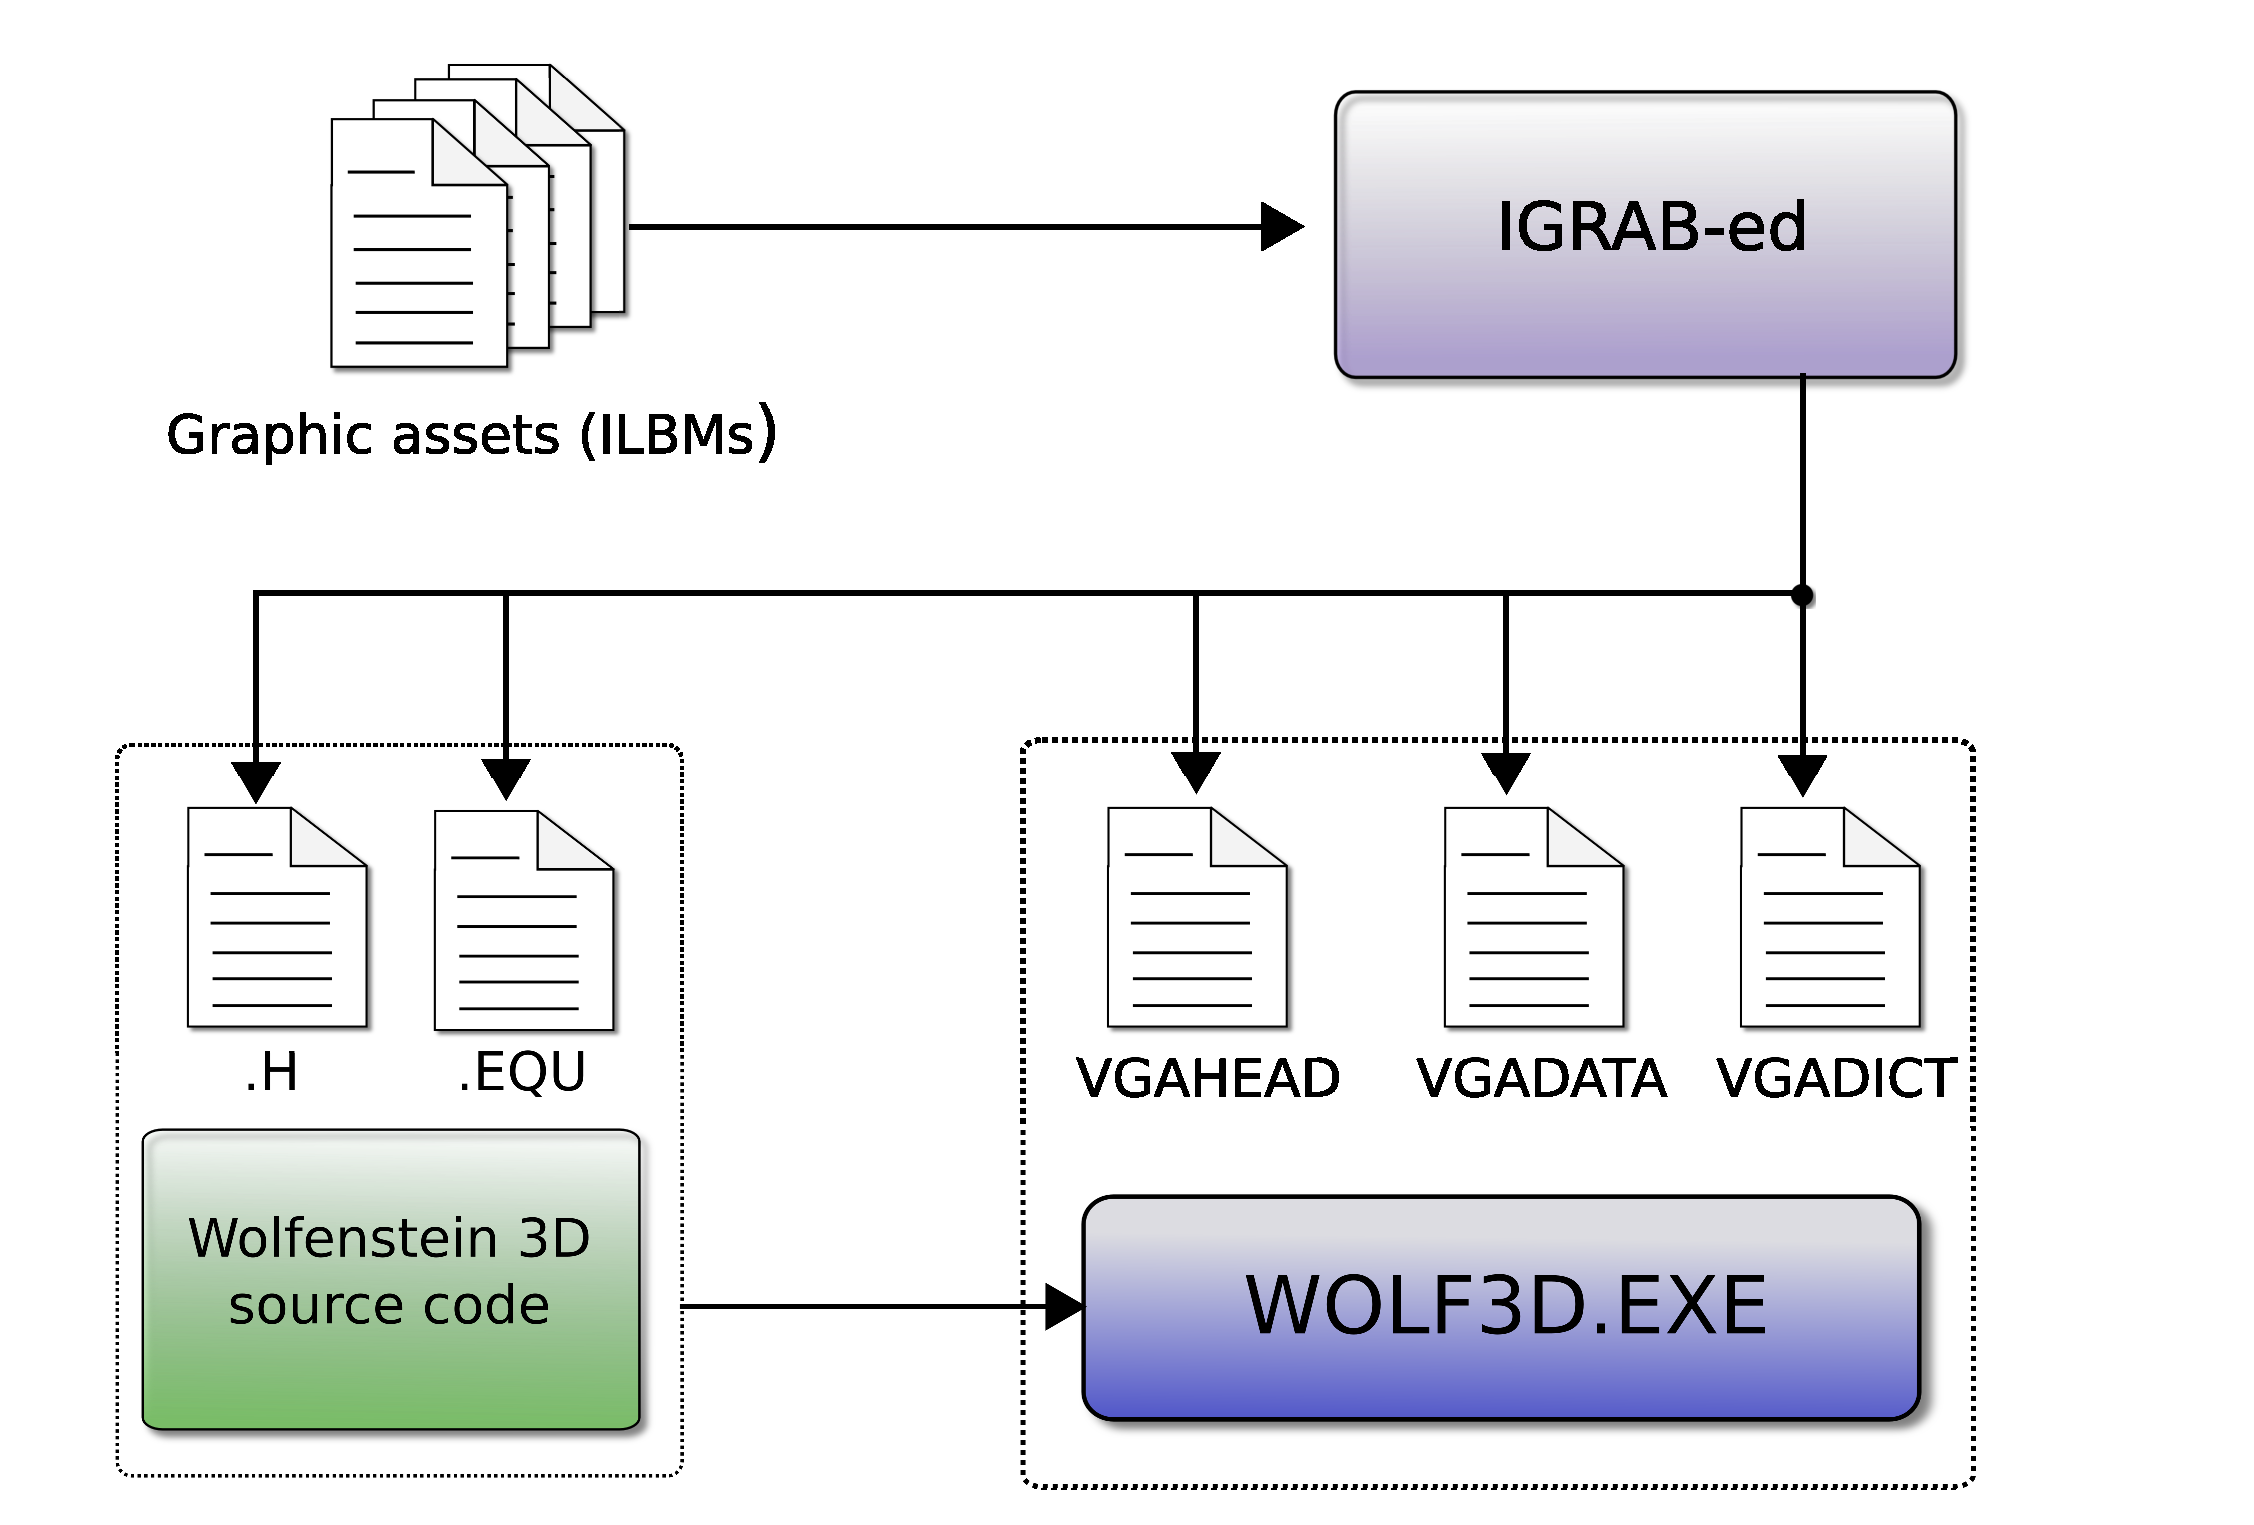
\includegraphics[scale=0.4]{imgs/drawing_plain.eps}
 \caption{Integer layout.} \label{fig:mips}
 \end{figure}

\section{Maps}
\section{Business}
\section{Sounds}
\section{Distribution}
	\subsection{Compression}
	\subsection{Shareware model}
\end{document}




